\documentclass[12pt, a4paper]{article}
\usepackage [T1]{fontenc}
\usepackage[margin=2.5cm]{geometry}
\usepackage[utf8]{inputenc}
\usepackage[english]{babel}
\usepackage{bm}
\usepackage{wasysym}
\usepackage{float}
\usepackage{pifont}
\usepackage{amsthm}
\usepackage{mathtools}
\usepackage[toc,page]{appendix}
\setcounter{tocdepth}{1}
\usepackage{listings}
\usepackage[cal=cm]{mathalfa}
\usepackage[version=3]{mhchem}
\usepackage{algorithmic}
\usepackage[nottoc]{tocbibind}
\usepackage[normalem]{ulem}
\usepackage{multirow}
\usepackage{tcolorbox}
\usepackage{adjustbox}
\usepackage{array}
\usepackage{tabularx}
\usepackage{longtable}
\usepackage{tabulary}
\usepackage{color}
\usepackage{colortbl}
\usepackage{gensymb}
\usepackage{pdfpages}
\usepackage{caption}
\usepackage{subcaption}
\usepackage{listings}
\usepackage{diagbox}
\usepackage{hyperref}
\usepackage[section]{placeins}
\usepackage{bbm}
\usepackage[linesnumbered,algoruled]{algorithm2e}

% Code format
\usepackage{minted}
\setminted{
	frame=lines,
	framesep=2mm,
	baselinestretch=1.2,
	%bgcolor=background,
	linenos,
	fontsize=\footnotesize,
	breaklines=true
}


% Math ops
\usepackage{amsmath,amssymb}
\DeclareMathOperator*{\argmax}{arg\,max}
\DeclareMathOperator*{\argmin}{arg\,min}
\DeclareMathOperator*{\EX}{\mathbb{E}}% expected value

\DeclarePairedDelimiter{\ceil}{\lceil}{\rceil}
\DeclarePairedDelimiter{\floor}{\lfloor}{\rfloor}

\newcommand{\dunderline}[1]{\underline{\underline{#1}}}
\newcommand{\euler}[1]{\ensuremath{\ \mathrm{e}^{#1}}}
\newcommand{\ma}[1]{\textbf{#1}}
\newcommand{\ve}[1]{\textbf{#1}}
\newcommand{\ap}[1]{\mathrm{\overline{#1}}}
\newcommand{\pp}[1]{\left( {#1} \right)}
\newcommand{\abs}[1]{\left|   {#1} \right|  }
\newcommand{\forn}[2]{{#1} \rightarrow {#2} \quad \text{for} \quad n \rightarrow \infty }
\newcommand{\forN}[2]{{#1} \rightarrow {#2} \quad \text{for} \quad N \rightarrow \infty }
\newcommand{\folg}[3]{ \{#1_{#3}\}_{#3 = #2}^{\infty} }
\newcommand{\folgc}[3]{ \{#1_{#3}\}_{#3 = #2}^{c} }
\newcommand{\ip}[2]{\langle{#1} , {#2}\rangle}

\newcommand{\RR}{ \mathbb{R} }
\newcommand{\NN}{ \mathbb{N} }
\newcommand{\CC}{ \mathbb{C} }
\newcommand{\for}{  \quad \text{for} \quad  }
\newcommand{\as}{  \quad \text{as} \quad  }

\usepackage{amsthm}
\usepackage{xcolor}
 

\theoremstyle{definition}
\newtheorem{definition}{Definition}[section]
\newtheorem{problem}{Problem}[section]
\newtheorem{theorem}{Theorem}[section]
\newtheorem{corollary}{Corollary}[theorem]
\newtheorem{lemma}[theorem]{Lemma}
\usepackage{hyperref}
\addbibresource{main.bib}
\author{Minh}
\begin{document}
	\begin{titlepage}
		\centering
		
\includegraphics[width=\textwidth]{KuLogo.png}
		\par\vspace{1cm}
		\vspace{1cm}

		{\scshape\Large Automatic Differentiation \\
			\par}

		\vspace{1.5cm}
		{\Large\itshape  Minh Duc Tran }\\
		\vspace{0.5cm}
		{\scshape\large cwz688 \\ \par}
		\vfill

		{\Large\scshape Master project \par}

		\vfill
		\par
		\vfill
		{\large \today\par}
	\end{titlepage}
	\newpage
\tableofcontents
\newpage 
\begin{abstract}
	Automatic diff is good
\end{abstract}
\section{Introduction}
Many important problems require taking derivatives to be solved. Such problems include 
Bundle Adjustment (BA) (cite) and XX. While finding the derivative for simple trivial functions 
can be done by hand. This method is accurate and often the 
fastest method when executed but it scales poorly for problems of real world relevance as 
finding the derivatives by hand is time consuming and can be error prone.  We hence seek to 
automate the process of finding these derivatives. \newline 

The simplest method to implement is \textit{numerical differentiation} methods 
but is slow in execution as it requires two evaluations per scalar derivative. 
It also suffers from numerical imprecision. A more precise method is 
\textit{symbolic differentiation}, which are often used in  ''mathematical'' languages
like Matlab, Mathematica or on your old TI-89.  This generates exact symbolic derivates, but 
is memory intensive and slow to compute. It can also not handle 
complex logic such as unbounded loops and hence is not appropriate for general computer programs. 
For solving most of these issues we turn to \textit{automatic differentiation}, which can 
compute exact derivatives for an arbitrary computer program. The caveat is however 
that the implementation must be carefully thought out. We will in this report
see how one can implement automatic differentiation in a way that minimizes 
the computational ....

\subsection{Motivation}


\section{Automatic differentiation}
Automatic differentiation (AD) relies on the fact every computer program, regardless of how complex it is, 
is a composition of arithmetic operations, like addition, multiplication etc. with well-defined derivatives. 
Along with the chain rule one can compute the derivative for any differentiable function written as a computer program.  
For example consider the composition of $n$ scalar functions:
$f(x) = f^n \circ f^{n-1} \circ \cdots \circ f^1 \circ x$. The chain then simply states that the derivate of 
$f$ w.r.t. $x$ is 
\begin{equation}
\frac{\partial f}{\partial x} = \frac{f^L}{f^{L-1}} \frac{f^{L-1}}{f^{L-2}} \cdots \frac{f^1}{x}
\label{eq:f}
\end{equation}
By formulating our function $f(x)$ as a program we are able to use AD to compute $\frac{\partial f}{\partial x}$ automatically. 
AD implementations usually has two distinct modes, forward- and reverse-mode.
The main difference between these two is in which direction the terms of each partial derivatives of the chain rule
are computed. For example in Eq. \ref{eq:f} forward-mode starts from the right most term, i.e. it first computes $\frac{f^1}{x}$
and traverses to the left. On the other hand does reverse-mode start from $\frac{f^L}{f^{L-1}}$ and accumulate to the right. \newline 
The formulating above is oversimplified for most AD problems and we in the general case 
have a multi-dimensional function $f : \mathbb{R}^n \to \mathbb{R}^m$  which would then have the $m\times n$  Jacobian matrix $J_f$:
\begin{figure}[H]
	$$ J_{f} = \left(\begin{matrix}
	\frac{\partial f_1}{\partial x_1} & \cdots & \frac{\partial f_1}{\partial x_n} \\
    \vdots & \ddots & \vdots \\
	\frac{\partial f_m}{\partial x_1} & \cdots  &  \frac{\partial f_3}{\partial x_n}\\
	\end{matrix}\right) $$
	\caption{$m\times n$ Jacobian matrix of layout $f : \mathbb{R}^n \to \mathbb{R}^m$}
\end{figure}
Given an input vector $x \in \mathbb{R}^n$  forward-mode evaluates $f$ once and computes a column of $J_f$. 
Hence to compute the entire Jacobian we need to perform $n$ evaluations of $f$.  
Techniques for reducing the number of passes can be done by performing an analysis on the columns of the 
Jacobian and partitioning them into as few structurally orthogonal groups as possible. 
This will be described in more details in Section \ref{sec:partitioning}.
Reverse-mode works in slightly different way. Given an output space vector $y \in \mathbb{R}^m$, a sweep will compute a 
row of $J_f$. Hence do we need to perform 1 evaluation of $f$ and $m$ reverse-mode sweeps.  We can now see the 
computational difference between the two modes. When $n \ll m$ forward-mode is more efficient and vice versa for $n \gg m$. 
Applications such as training a neural networks usually have large input dimensions $n$ compared to output dimension $m$ and hence are 
libraries like Tensorflow\footnote{\url{https://www.tensorflow.org/}}  reverse-mode based. One downside to reverse-mode is that 
it requires access to intermediate variables computed during the evaluation and hence require more memory.  


\subsection{Forward-mode implementations}
The implementation of forward-mode can be done with two strategies:
\subsubsection*{Source code transformation}
One of the oldest methods for AD is source code transformation. Here an AD tool, (or preprocessor), rewrites our function that we wish to 
compute the derivative of. A preprocessor then applies the differentiation rules as prescribed by the elementary operators and chain rules, 
and returns the augmented source code function which now includes statements for computing the derivatives. The resulting source
code can be compiled and executed as usual. There are few examples of such implementations. 
For example has Tangent\cite{DBLP:journals/corr/abs-1711-02712} implemented AD support for a subset of the Python language, 
while Tapenade has AD tools for transforming C and Fortran functions. The major downsides of source code transformation is that 
they can only use information available at compile time and developing the tools is non-trivial and requires a lot of effort. 
Therefore do we often see that AD are implemented using operator overloading. 
	
\subsubsection*{Operator overloading}
Operator overloading (OO) is far more common and simpler to implement.
Forward-mode OO is usually implemented using \emph{dual numbers}, which extends the real numbers 
of the programming language by a differential component. The real number operators are then lifted to
operate on the dual numbers and provide a powerful abstraction, where the details of derivatives can 
be hidden away from the programmer. Furthermore can implementations usually be an embedded DSL in form of a library 
within a more general host language. These DSL can then leverage the constructs and features of the host language and can be imported
as any other library. This ensures a flexible and portable advantage of having such an embedded DSL. Examples of such DSL libraries are 
\texttt{Julia ForwardDiff}\cite{RevelsLubinPapamarkou2016} and \texttt{Stan Math}\cite{DBLP:journals/corr/CarpenterHBLLB15}. 
The next section provides an example of how forward-mode AD with operator overloading can be applied to a simple
function. 



\subsubsection*{Example}
Consider the  function $f:\mathbb{R}^2 \to \mathbb{R}$ defined by $f(x_1, x_2) = x_1 \cdot x_2 + \sin x_1$.
We show how one can numerical compute the partial derivative $\frac{\partial}{\partial x_1} \left( x_1 \cdot x_2 + \sin x_1 \right)$ 
of such a function by using forward-mode AD with operator overloading. With operator overloading each
variable $x$ is augmented with it's \emph{numerical} derivate value, which we denote by a dot, i.e. for a variable $x_1$
we denote it's derivate value as $\dot{x}_1$. The operations that can be performed on such a variable 
are now a function pair of the operation itself and it's derivative expression w.r.t. it's inputs. For example for 
scalar multiplication on $x_1$ and $x_2$ the  derivative expression is $x_1 \cdot \dot{x}_2 + x_2 \cdot \dot{x}_1$ as we want to be able to compute the derivative of either $x_1$ or $x_2$. Hence we have that a scalar value is stored as $(x, \dot{x})$ and a multiplication
operation on such a type has the operator pair $(x_1 \cdot x_2; x_1 \cdot \dot{x}_2 + x_2 \cdot \dot{x}_1) $.
As the function is evaluated with forward-mode AD,  also called a forward sweep,
the derivatives are then automatically evaluated along and combined through the chain rule. 
The independent variable which one wants to differentiate with respect to is decided by setting a \emph{seed} for that variable.
For example as we want to differentiate w.r.t. $x_1$ we set $\dot{w}_1 = \frac{\partial x_1}{\partial x_1} = 1$ and $\dot{w}_2 = \frac{\partial x_2}{\partial x_2} = 0$, where we define $\dot{w}_i$ for sub-expression $i$. With these seeds set; Table \ref{tab:example}  shows a symbolic forward sweep of $f$ for computing $\frac{\partial}{\partial x_1} \left( x_1 \cdot x_2 + \sin x_1 \right)$. 
%Some of the derivate identities used in this example are $\frac{\partial x}{\partial x} = 1$ and $\frac{\partial \sin x}{\partial x} = \cos x$.  
\begin{table}[H]
	\centering 
	\begin{tabular}{l|l}
		Operations to evaluate $f$ & Operations to evaluate the derivative          \\ \hline \hline 
		$w_1 = x_1$               & $\dot{w}_1 = 1$ (seed)                                  \\
		$w_2 = x_2$               & $\dot{w}_2 = 0$ (seed)                                  \\
		$w_3 = w_1 \cdot w_2$     & $\dot{w_3} = w_2 \cdot \dot{w}_1 + w_1 \cdot \dot{w}_2$ \\
		$w_4 = \sin w_1$          & $\dot{w}_4 = \cos w_1  \cdot  \dot{w}_1$                        \\
		$w_5 = w_3 + w_4$         & $\dot{w}_5 = \dot{w}_3 + \dot{w}_4$                    
	\end{tabular}
\caption{Example of a symbolic forward pass for forward-mode AD for computing $\frac{\partial}{\partial x_1} \left( x_1 \cdot x_2 + \sin x_1 \right)$}
\label{tab:example}
\end{table}
By setting the input values, $x_1 = 1$ and $x_2 = 2$ we can numerically evaluate our derivative as:
\begin{equation}
\frac{\partial f}{\partial x_1} = w_2 \cdot \dot{w}_1 + w_1 \cdot \dot{w}_2 + \cos w_1  \cdot  \dot{w}_1 =  2 \cdot 1 + 1 \cdot 0 + \cos 1 \cdot 1 = 2.5403
\label{eq:seeds}
\end{equation} 
Which is the result we would also have obtained through differentiation by hand. 
If we wanted to compute the Jacobian of $f$ we also need to compute $\frac{\partial f}{\partial x_2}$  
and we would need to change our seeds to $\dot{w}_1 = 0$ and $\dot{w}_2 = 1$ 
and perform another forward sweep. 
The reader may wonder why we can't set both seeds to 1 and settle for single forward sweep. 
Consider the operation $x_1 \cdot x_2$ with the two input values, $x_1$ and $x_2$ with the derivative expression
$x_1 \cdot \dot{x}_2 + x_2 \cdot \dot{x}_1$. If we then set both seeds to 1, both terms will then contribute to 
the partial derivative, i.e. there is interleaving, which would result in neither derivatives being correct. For example in Eq. \ref{eq:seeds}
will the middle term now contribute to the resulting derivative for $\frac{\partial f}{\partial x_1}$. Hence do we need a separate forward sweep for each
independent variable that we wish to compute the derivative of. 
\subsubsection{Problems}
\subsubsection*{Exploiting sparsity of the Jacobian}
One common problem for many applications of AD is that many elements of the Jacobian
are zeros and as such said to be sparse. Such sparsity in the Jacobian can 
be exploited for more efficient computations by using fewer forward passes. The problem
of reducing the number of forward passes can be formulated as a matrix partitioning problem. 
As an example consider the sparse Jacobian for a function $f: \mathbb{R}^n \to  \mathbb{R}^m$ with $m=n=5$ in Figure \ref{fig:jacobian}. By not exploiting the sparsity of the Jacobian, forward-mode AD requires $n=5$ forward passes to compute the Jacobian.
\begin{figure}[H]
	$$ \left(\begin{matrix}
    j_{11} & j_{12} & 0 & 0 & j_{15} \\
    0 & 0 & j_{23} & 0 & 0 \\
    0 & j_{32} & j_{33} & j_{34} & 0 \\
    j_{41} & 0 & 0 & 0 & 0 \\
    0 & 0 & 0 & j_{54} & j_{55} 
	\end{matrix}\right) $$
	\caption{Jacobian from \texttt{f} for $m=n=5$}
	\label{fig:jacobian}
\end{figure}
However it's possible in this case to exploit the sparsity to reduce the number of forward passes down to three. Consider a subset of the columns of the Jacobian such that no two columns have a non-zero in a common row. Such a subset of columns are said to be \emph{structurally orthogonal}. Formulated differently, is every pair of columns in such a subset, pairwise orthogonal to each other and is independent of each other in the numerical values of the non-zeros. In the example above are columns 1 and 3 structurally orthogonal, as well as columns 1 and 4; and 3 and 5. By finding the minimum number of structurally orthogonal subsets we are able to reduce the number of forward passes. 
The problem can be formulated as:
\begin{problem}
	Given the sparsity structure of an $m \times n$ matrix A, find a structurally orthogonal partition of its columns that has the \emph{fewest} groups.
	\label{prob:p1}
\end{problem}
For example if we partition the Jacobian above into 3 subsets $\{\{1,4\}, \{2\}, \{3,5\}\}$ we are able to compute the compressed Jacobian with just 3 passes. Without loss of information our compressed Jacobian will look like: 
\begin{figure}[H]
		$$ \left(\begin{matrix}
	{\color{blue} j_{11}} & {\color{red} j_{12}} & {\color{green} 0 }        &  {\color{blue} 0 }       & {\color{green} j_{15}} \\
	{\color{blue} 0}        & {\color{red} 0 }       & {\color{green} j_{23}}  &  {\color{blue} 0 }      & {\color{green} 0} \\
	{\color{blue} 0}        & {\color{red}j_{32}} &  {\color{green} j_{33}}  & {\color{blue} j_{34}} & {\color{green} 0 } \\
	{\color{blue} j_{41}} & {\color{red} 0 }       & {\color{green} 0 }         & {\color{blue} 0 }        & {\color{green} 0} \\
	{\color{blue} 0 }       & {\color{red} 0 }       & {\color{green} 0 }         & {\color{blue} j_{54}} & {\color{green} j_{55} }
	\end{matrix}\right) \Rightarrow \left(\begin{matrix}
	{\color{blue} j_{11}} & {\color{red} j_{12}} & {\color{green} j_{15}} \\
	{\color{blue} 0} & {\color{red} 0} & {\color{green} j_{23}} \\
	{\color{blue} j_{34}} & {\color{red} j_{32}} & {\color{green} j_{33}}  \\
	{\color{blue} j_{41}} & {\color{red} 0} & {\color{green} 0}  \\
	{\color{blue} j_{51}} & {\color{red} 0} & {\color{green} j_{55}} &  
	\end{matrix}\right) $$
	\caption{Compressed Jacobian from \texttt{f} for $m$ = $n$ = $5$ with partitioning $\{\{1,4\}, \{2\}, \{3,5\}\}$}
	\label{fig:Jacob_partition}
\end{figure}
In practice it means that we've reduced the size of the Jacobian from $5 \times 5$ to a compressed Jacobian of size $3 \times 3$ and in this case it's clear that it's the minimum size that we can reduce to. Finding such an optimal partitioning can be done
by modelling the problem as a graph colouring problem.  Unfortunately is 
the general graph-colouring problem known to be NP-hard, so algorithms presented here are based on effective heuristics. Next section presents simple algorithms for matrix partitioning of Jacobian. For a more thorough presentation it is refereed to \cite{Jacobian}, which also presents algorithms for 
partitioning Hessians and much more. The next section shows how we can formulate Problem \ref{prob:p1} as a 
Graph Colouring problem and presents algorithms for unidirectional\footnote{Here unidirectional means only partitioning over columns, unlike bidirectional which is partitioning over rows and column} matrix partitioning of Jacobian matrices. 


\subsection{Graph Colouring for matrix partitioning}
\label{sec:partitioning}
In the following I assume that the reader is familiar with basic graph theory terminology. 
This section's results are based on Chapter 1-3 in \cite{Jacobian} and here
we  only present the most essential definitions and results used in the algorithm presented 
below for matrix partitioning with graph colouring. The proofs of the presented theorems and lemmas 
can also be found in \cite{Jacobian} and are here omitted for brevity.
We start with a graph colouring definition. 
\subsubsection*{Distance-k Graph Colouring}
\begin{definition}
A \textit{distance-k} vertex colouring of a graph $G = (V,E)$ is a mapping $\phi : V \to \{1,2,..., p\}$ such that $\phi(u) \not= \phi(v)$ whenever vertices $u$ and $v$ are distance-$k$ neighbours. The least possible number of colours required to colour $G$ is called the chromatic number of $G$ and is denoted $\chi_k(G)$. Furthermore is a distance-$k$ colouring of $G = (V,E)$ called \emph{partial} if it only covers a proper subset $W \subset V$ of the vertices. We then have that $\phi: W \to \{1,2, \cdots, p\}$ is a mapping such that  $\phi(u) \not= \phi(v)$ whenever vertices $u, v \in W$ are distance-$k$ neighbours in $G$.  
\end{definition}

\subsubsection*{The power of a Graph}
\begin{definition}
The \emph{k}th power of a graph $G$ is the graph $G^k$ whose vertex set is the same as that of $G$ and whose edge set consists of pairs of vertices $(u,v)$ whenever vertices $u$ and $v$ are distance-$k$ neighbours in G. 
This leads us to the  lemma:
\end{definition}
\begin{lemma}
A mapping $\phi : V \to \{1,2,..., p\}$ is a distance-$k$ coloring of $G$ if and only if it is a distance-1 colouring of $G^k$
\end{lemma}

\subsubsection*{Representing Matrices Using Graphs}
%Here's we will present different graph presentations of the sparsity structure of matrices. 
For a matrix $A$ we'll denote the $i$th row as $r_i$ and the $j$th column
as $c_j$. Finally is the $(i,j)$ entry of A denoted as $a_{ij}$. We now show how we can
construct a bipartite graph representation from a matrix $A$. \newline 
\textbf{Bipartite Graphs}: Let $A$ be an $m \times n$ matrix with rows $r_1, r_2, \dots, r_m$ and columns $c_1, c_2, \dots, c_n$. The bipartite graph of $A$, denoted $G_b(A)$, is defined as $G_b(A) = (V_1, V_2, E)$, where $V_1 = \{r_1, r_2, ..., r_m\}$, $V_2 = \{c_1, c_2, ..., c_n\}$ and $(r_i, c_j) \in E$ whenever $a_{ij}$ is non-zero for $1 \leq i \leq m, 1 \leq j \leq n$.  An example of the bipartite representation is shown in Figure \ref{fig:bipartite}. 
\begin{figure}[H]
	\centering
	\begin{subfigure}{0.45\linewidth}
	$$ \left(\begin{matrix}
{\color{blue} a_{11}} & {\color{red} a_{12}} & {\color{green} 0 }        &  {\color{blue} 0 }       & {\color{green} a_{15}} \\
{\color{blue} 0}        & {\color{red} 0 }       & {\color{green} a_{23}}  &  {\color{blue} 0 }      & {\color{green} 0} \\
{\color{blue} 0}        & {\color{red} a_{32}} &  {\color{green} a_{33}}  & {\color{blue} a_{34}} & {\color{green} 0 } \\
{\color{blue} a_{41}} & {\color{red} 0 }       & {\color{green} 0 }         & {\color{blue} 0 }        & {\color{green} 0} \\
{\color{blue} 0 }       & {\color{red} 0 }       & {\color{green} 0 }         & {\color{blue} a_{54}} & {\color{green} a_{55} }
\end{matrix}\right) $$
	\end{subfigure}
	 $\Rightarrow$ \hfill 
	\begin{subfigure}{0.45\linewidth}
	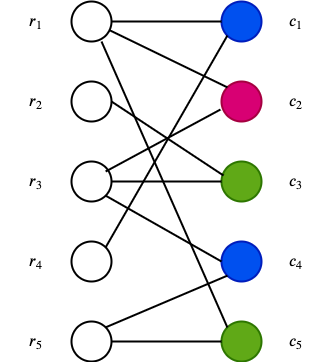
\includegraphics[width=0.6\textwidth]{pics/bipartite.png} 
	\end{subfigure}
     \caption{Example of a bipartite representation of the matrix partitioning from Figure \ref{fig:Jacob_partition}}
	\label{fig:bipartite}
\end{figure}
Note that the size of graph is proportional to size of an $m \times n$ matrix A, i.e. we have $\vert V_1 \vert  + \vert V_2 \vert = m + n$ vertices and $\vert E \vert = nnz(A)$, where $nnz(A)$ denotes the number of non-zero entries of $A$. Having set our preliminaries we are now able to express Problem
\ref{prob:p1} as a Graph Colouring Problem. We make us of the following theorem:
\begin{theorem}
	Let $A$ be an $m \times n$ matrix and $G_b(A) = (V_1, V_2, E)$ be its bipartite graph representation. A mapping $\phi$ is a partial distance-2 coloring of $G_b(A)$ on $V_2$ if and only if $\phi$ induces a structurally orthogonal partition of the columns of A. 
	\label{th:th1}
\end{theorem}
The reader may verify that the partitioning in Figure \ref{fig:bipartite} indeed satisfies the partial distance-2 colouring of 
it's bipartite representation. An important corollary of Theorem \ref{th:th1} is 
\begin{corollary}
	Let $\chi_2(G_b, V_2)$ denote the chromatic number for a partial distance-2 colouring of $G_b(A) = (V_1, V_2, E)$  on $V_2$. 
	Then $\chi_2(G_b, V_2)$ is the minimum number of forward passes required to compute the Jacobian and hence is a lower bound. 
	\label{col:minimum}
\end{corollary}
Corollary \ref{col:minimum} simply states that if we can find the minimum number of colours required for a partial distance-2 colouring of $G_b(A) = (V_1, V_2, E)$  on $V_2$  then we've found the optimal partition for computing the  Jacobian in the fewest number of forward passes. From Theorem \ref{th:th1} we are now able to formulate the equivalent graph colouring problem from Problem \ref{prob:p1}:
\begin{problem}
	Given the bipartite graph $G_b(A) = (V_1, V_2, E)$ representing the sparsity structure of an $m \times n$ matrix $A$, find a partial distance-2 colouring of $G_b(A)$ on $V_2$ that uses the fewest colours. 
\end{problem} 


\subsubsection{A greedy distance-2 Colouring Algorithm}
An algorithm for finding a greedy distance is shown in Algorithm \ref{alg:greedy2}.\newline 
\begin{algorithm}[H]
	\SetAlgoLined
	\KwIn{$G_b = (V_1, V_2, E)$ }
	\KwResult{A partitioning of the co}
	Let $v_1, v_2, ..., v_{\vert V_2 \vert}$ be a given ordering of $V_2$\;
	Initialize \texttt{forbiddenColours} with some some value $a \not\in V_2$\;
	\For{$i \leftarrow 1$ \texttt{to} $\vert V_2 \vert$}
	{
		\ForEach{$w \in N_1(v_i)$}
		{
			\ForEach{\texttt{coloured vertex} $x \in N_1(w)$}
			{
				\texttt{forbiddenColours}$\lbrack \texttt{color} \lbrack x \rbrack \rbrack \leftarrow v_i$
    		}
	    }  
        \texttt{colour}$\lbrack v_i \rbrack$ $\leftarrow \min \{ c > 0 : \texttt{forbiddenColours}\lbrack c \rbrack \not= v_i \}$
    }	
	\caption{A greedy partial distance-2 colouring algorithm}
	\label{alg:greedy2}
\end{algorithm}




\section{Implementation in Futhark}
To see how we can make use of the results from previous section 
in Futhark we implement the colouring algorithm and show how easily
we can apply it to a Jacobian to reduce the number of forward-passes. 
Implementing graph colouring for matrix column partitioning is fairly simple. We also, without any modifications, use the already implemented forward-AD library, \url{https://github.com/diku-dk/futhark-ad}. All the code can be found in Appendix A. 
Consider the stencil function in Listing \ref{lst:tridiag} and note that every output value only depends on at most three different input values.
\begin{listing}[H]
\begin{minted}{haskell}
let f xs =
  let n = length xs
  in map  (\i -> if i == 0 then 
                     f32_dual.(xs[0] + xs[1])
                 else if i == n - 1 then
                     let x1 = xs[n - 2]
                     let x2 = xs[n - 1]
                     in f32_dual.(x1 + x2)
                 else
                     let x1 = xs[i-1]
                     let x2 = xs[i]
                     let x3 = xs[i+1]
                     in f32_dual.(x1 + x2 + x3)) (iota (n))
\end{minted}
\caption{Stencil function with a tri-diagonal Jacobian}
\label{lst:tridiag}
\end{listing}
The Jacobian of such a function when the input dimension is $n= 5$, is shown in Figure \ref{fig:tridiag}. Note that 
the Jacobian is very sparse, regardless of the input dimension, and only contains elements along the
tri-diagonal and zeros elsewhere.  
\begin{figure}[H]
	$$ J_{f} = \left(\begin{matrix}
	\frac{\partial f_1}{\partial x_1} & \frac{\partial f_1}{\partial x_2} & 0 & 0 & 0 \\
	\frac{\partial f_2}{\partial x_1}& \frac{\partial f_2}{\partial x_2} & \frac{\partial f_2}{\partial x_3} & 0 & 0\\
	0 & \frac{\partial f_3}{\partial x_2} & \frac{\partial f_3}{\partial x_3} & \frac{\partial f_3}{\partial x_4} & 0\\
	0 & 0 & \frac{\partial f_4}{\partial x_3} & \frac{\partial f_4}{\partial x_4} & \frac{\partial f_4}{\partial x_5} \\
	0 & 0 & 0 & \frac{\partial f_5}{\partial x_4} & \frac{\partial f_5}{\partial x_5}
	\end{matrix}\right) $$
	\caption{Jacobian from \texttt{f} in Listing \ref{lst:tridiag} for $n=5$}
	\label{fig:tridiag}
\end{figure}
For a simple implementation of forward-mode AD we'll normally use
$n$ forward passes to compute the Jacobian. While we are able to compute each 
forward sweep in parallel in Futhark on GPU, most of the computations are wasted.
However by applying the techniques from previous Section, we able to only use $3$ forward passes
of the function \texttt{f} \emph{regardless} of the input dimension $n$.  
Recall that we able to transform any $m\times n$ matrix $A$ into a bipartite graph 
representation by letting the row be set of vertices of $V_1$ and the columns be $V_2$. 
%that we only need to find a distance-2 colouring of the vertices of $V_2$.
We use an adjacency matrix to represent our bipartite graph as such:
\begin{figure}[H]
	$$ G_f = \left(\begin{matrix}
     1 & 1 & 0 & 0 & 0 \\
	1 & 1 & 1 & 0 & 0\\
	0 & 1 & 1 & 1 & 0\\
	0 & 0 & 1 & 1 & 1 \\
	0 & 0 & 0 & 1 & 1
	\end{matrix}\right) $$
	\caption{Adjacency matrix, $G_f$ derived from \texttt{$J_f$} in Figure \ref{fig:tridiag} with rows representing vertices of $V_1$ and columns representing vertices of $V_2$}
\end{figure}
The implementation of the greedy distance-2 colouring in Futhark is shown in Listing \ref{lst:greedy2}. Note that the implementation is sequential in the outer-most loop, but is parallel inside the loop-body.  
A  discussion of parallel colouring algorithms are beyond the scope of this project. 
%but the reader is referred to \cite{parallelgraph}. 
\begin{listing}[H]
	\begin{minted}{haskell}
let greedy_distance_2_coloring [m][n] (G:[m][n]i32) : [n]i32 =
  let coloring = replicate n 0
  let colored = replicate (n*m) (false) 
  let forbiddenColors = replicate (min max_colors n) (n+1)
  let (coloring, _, _) =
    loop (coloring, forbiddenColors, colored) for j < n do
    let N_v = filter (>=0) <| tabulate m (\i -> if G[i,j] == 1 then i else (-1))  
    let colored_index_N_w = flatten <| map (\j' -> tabulate m (\i -> if unsafe colored[j' * m + i] then i else (-1))) N_v
    let colored_index_N_w = filter (>= 0) colored_index_N_w
    let color_idx = map (\i -> coloring[i]) colored_index_N_w   
    let forbiddenColors' = scatter forbiddenColors color_idx (replicate (length color_idx) j)
    let idx = map (\i -> i * m + j) N_v
    let coloring[j] = argmin j forbiddenColors'
    let colored' = scatter colored idx (replicate (length idx) true)
    in (coloring, forbiddenColors', colored')
  in coloring
	\end{minted}
	\caption{Implementation of Algorithm \ref{alg:greedy2} in Futhark}
	\label{lst:greedy2}
\end{listing}
Having a colouring vector for $V_2$ we are now able to compute the 
seed matrix as such. 
\begin{listing}[H]
\begin{minted}{haskell}
let compute_seed_matrix [n] (coloring:[n]i32) :[][]f32 =
  let max_col = maximum coloring
  in tabulate max_col (\i -> map (\c -> if c == i then 1 else 0) coloring)
\end{minted}
\end{listing}

\subsection{Limitations}
While the given example results in an optimal and impressive result of 
only requiring 3 forward passes regardless of the input size 
it's considered a special case. In the general case we might 
run into other issues such as:
\begin{itemize}
	\item The presented graph colouring algorithm is an approximation algorithm. 
	While it performs reasonable in practice it does rarely yield an optimal colouring
	\item Data dependencies
	\item Still need to evaluate $F$ at least once fully. 
\end{itemize}


\section{Discussion}




\section{Conclussion}




















\newpage 
\newpage 


\section{Legacy stuff}
\subsection{Example: Data-independent sparsity}

This section is based on Julia's approach to sparse AD computation. 
Link: \url{https://github.com/JuliaDiffEq/SparseDiffTools.jl}. 

Below is a function which performs a 1D-convolution on the input array $x$ of dimension $n$. 
The Jacobian of such a function is the tri-diagonal matrix shown in Figure \ref{fig:tridiag}. 
\begin{minted}{C}
int* f (int* x, int n) {
retval = malloc(sizeof(int) * n);
for (int i = 1; i < n - 1; i++) {
retval[i] = x[i-1] + x[i] + x[i+1];
}
retval[0] = x[0] + x[1];
retval[n-1] = x[n-1] + x[n-2];
return retval;
}
\end{minted}
\begin{figure}[H]
	$$ J_{f} = \left(\begin{matrix}
	\frac{\partial f_1}{\partial x_1} & \frac{\partial f_1}{\partial x_2} & 0 & 0 & 0 \\
	\frac{\partial f_2}{\partial x_1}& \frac{\partial f_2}{\partial x_2} & \frac{\partial f_2}{\partial x_3} & 0 & 0\\
	0 & \frac{\partial f_3}{\partial x_2} & \frac{\partial f_3}{\partial x_3} & \frac{\partial f_3}{\partial x_4} & 0\\
	0 & 0 & \frac{\partial f_4}{\partial x_3} & \frac{\partial f_4}{\partial x_4} & \frac{\partial f_4}{\partial x_5} \\
	0 & 0 & 0 & \frac{\partial f_5}{\partial x_4} & \frac{\partial f_5}{\partial x_5}
	\end{matrix}\right) $$
	\caption{Jacobian from \texttt{f} for $n=5$}

\end{figure}
The sparsity of the Jacobian in this case is independent of the data, e.g. $x_1$ will always be independent of $f_5$ 
or more generally the off tri-diagonal elements will always be zero. 
Of course the case where the input value is zero, e.g. $x_1 = 0$  the entry $\frac{\partial f_1}{\partial x_1}$ will also be zero, which would then be \emph{data} dependent.

\subsection{Example: Bundle Adjustment - Data-dependent}
For a data-dependent example we use  Bundle Adjustment \footnote{Link to Wiki} as example and 
show that the layout of the Jacobian depends on how we represent our data as shown in Figure \ref{fig:jacobian-matrix-for-a-bundle-adjustment-problem-con-sisting-of-3-cameras-and-4-points}.
Note that for showing the natural sparsity of the Jacobian we have to represent the input data as one long vector
i.e. our input data has the form $\lbrack \texttt{cam1} \ \texttt{cam2} \ \texttt{cam3}\ X_1\ X_2\ X_3\ X_4 \rbrack $, 
where only one pair of \texttt{camX} and $X_i$ are non-zero for each data-row. 
The Jacobian sparsity pattern hence depends on the input, for example if we swap the columns \texttt{cam1} and \texttt{cam2}, keeping all else the same,
the sparsity pattern of the Jacobian also changes. 
\begin{figure}[H]
	\centering
	%\includegraphics[width=0.7\linewidth]{../../../Desktop/Jacobian-matrix-for-a-bundle-adjustment-problem-con-sisting-of-3-cameras-and-4-points}
	\caption{Data dependent sparse matrix stemming from Bundle Adjustment (Stolen from  \url{https://www.researchgate.net/figure/Jacobian-matrix-for-a-bundle-adjustment-problem-con-sisting-of-3-cameras-and-4-points_fig1_284154527})}
	\label{fig:jacobian-matrix-for-a-bundle-adjustment-problem-con-sisting-of-3-cameras-and-4-points}
\end{figure}


\subsection{Sparsity w.r.t. performance}
For Forward-mode AD we can reduce the computation of both types of sparsity with a \texttt{colour} vector, 
which  denotes which input parameters are independent (or dependent) of each other. 
This corresponds to solving a graph-colouring problem.
For example for the function \texttt{f} above we can use a color vector 
with three colours as each output value depends on at most three input values. 
A colour vector for $n=5$ could then be $\lbrack c_0, c_1, c_2, c_1, c_0\rbrack$ where input values with the 
same colour can be computed during the same forward-sweep, so we reduce the number of 
forward calls to the number of colours used. Worth noting is that \texttt{f}'s colour vector 
\emph{always}  contains 3 colours; independent of $n$ so the number of forward calls 
is effectively reduced by  $n-3 + 1$ in this case. (Plus one since we need to compute the colour vector)\newline 
For finding the colour-vector we can perform a forward sweep of the function 
with some random input and use some underlying data-structure to solve the graph-colouring problem. 
Alternatively can one let the user provide the color vector. 

\subsubsection{Bundle Adjustment revisited}
For Bundle Adjustment we can also use the same approach by seeding the forward sweep 
with the camera and point data. Using the data it's possible to figure out the dependencies and generate a 
coloring, which in this case would be a matrix, one for each data-row. 
In stochastic gradient descent methods, like used Bundle Adjustment, this color vector can provide a speed-up on subsequent 
computations of the Jacobian. 
However if the data is only used once, this approach requires that we compute the coloring again and again
and hence would not be very efficient. 



\subsection{Sparsity w.r.t. Memory}
Julia and STAN uses a sparse data structures but to my knowledge not feasible in Futhark?
Need more time to look into this. 

\newpage
\nocite{*}
\printbibliography


\end{document}